\section{The Components of the Jeliot~3 System}
\label{sec:The_Components_of_the_Jeliot_3_System}


\subsection{User Interface}
\label{sec:User_Interface}

The design of the user inteface is a crucial aspect in the tool for novice computer user.
We used the user interface design from Jeliot 2000 as it was found usable and simple for novices \citep{Levy2003}.
We have just added extra menus and short keys to make the lecture use of
the software smoother. Moreover, the line numbering was added to the code editor and view to
make the referencing to the code easier. The user interface of Jeliot~3 and its layout is
illustrated in the Figures~\ref{fig:jeliot3_UI_structure}.

- Picture of the user interface.

\begin{figure}[!htb]
\begin{center}
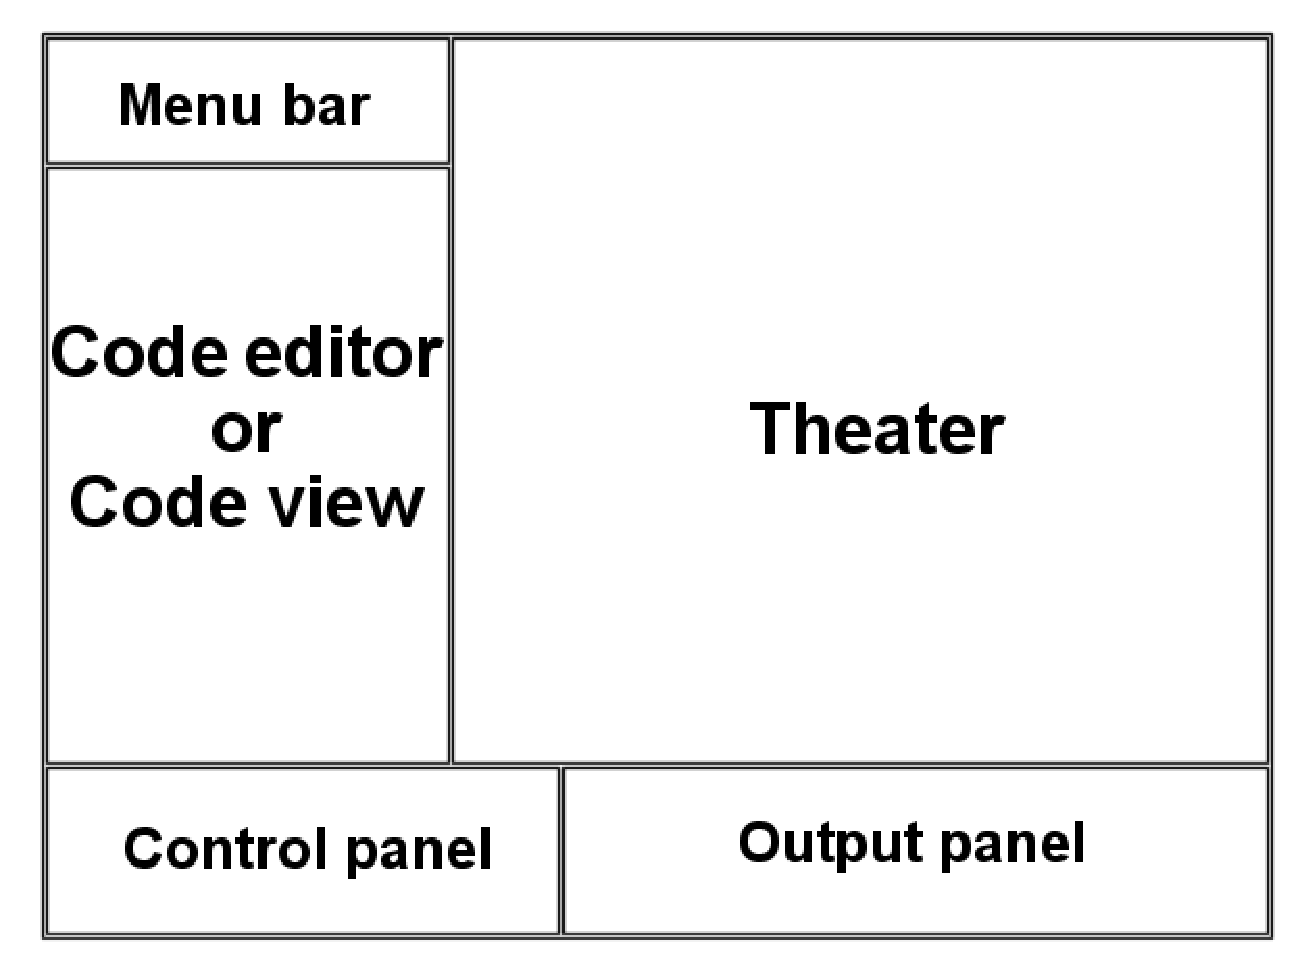
\includegraphics[height=10cm]{jeliot3_UI_structure.eps}
\caption{The structure of user interface in Jeliot~3.}
\label{fig:jeliot3_UI_structure}
\end{center}
\end{figure}


\subsection{Visualization Engine}
\label{sec:Visualization_Engine}




\subsection{DynamicJava}
\label{sec:DynamicJava}

Dynamic Java is a Java source code interpreter written in Java. This application is open source and can be freely obtained . At the moment, DynamicJava is almost fully compliant with Java specifications and supports multi-threading. Due to the lack of documentation (nothing is provided except an API documentation done by JavaDoc) it was necessary to take a look to the source code of the software to understand its beh